\documentclass[11pt]{article}
\usepackage[T1]{fontenc}
\usepackage[utf8]{inputenc}
\usepackage{newpxtext}
\usepackage[margin=1in,headheight=15pt]{geometry}
\usepackage{microtype}
\usepackage{amsmath,amsthm,mathtools}
\usepackage{newpxmath}
\usepackage{xcolor,graphicx,booktabs,array,float,xurl}
\usepackage[most]{tcolorbox}
\usepackage{enumitem,fancyhdr}
\usepackage[colorlinks=true,linkcolor=blue!45!black,citecolor=blue!45!black,
 urlcolor=blue!45!black,pdftitle={A sum-of-squares proof of Ulas's real-zero conjecture},
 pdfauthor={Research note prepared with ChatGPT}]{hyperref}
\usepackage[nameinlink,noabbrev]{cleveref}
\definecolor{ink}{HTML}{17354A}
\definecolor{accent}{HTML}{176B73}
\pagestyle{fancy}
\fancyhf{}
\fancyhead[L]{\small\textsc{Stern polynomials: positivity and zero geometry}}
\fancyhead[R]{\small Research note}
\fancyfoot[C]{\thepage}
\renewcommand{\headrulewidth}{0.3pt}
\setlength{\parskip}{4pt}
\setlength{\parindent}{1.2em}
\setlist{nosep,leftmargin=1.6em}
\numberwithin{equation}{section}
\newtheorem{theorem}{Theorem}[section]
\newtheorem{lemma}[theorem]{Lemma}
\newtheorem{proposition}[theorem]{Proposition}
\newtheorem{corollary}[theorem]{Corollary}
\theoremstyle{definition}
\newtheorem{remark}[theorem]{Remark}
\newcommand{\Z}{\mathbb Z}
\newcommand{\Q}{\mathbb Q}
\newcommand{\R}{\mathbb R}
\newcommand{\C}{\mathbb C}
\newcommand{\F}{\mathbb F}
\newcommand{\Repart}{\operatorname{Re}}
\newcommand{\Impart}{\operatorname{Im}}
\newcommand{\lc}{\operatorname{lc}}
\newcommand{\ord}{\operatorname{ord}}
\newcommand{\zetaSix}{\zeta}
\newcommand{\W}{W}
\newtcolorbox{statusbox}{enhanced,breakable,colback=ink!3,colframe=ink!35,
 boxrule=0.4pt,arc=1.5mm,left=3mm,right=3mm,top=2mm,bottom=2mm}
\begin{document}
\thispagestyle{empty}
\begin{center}
 {\small\sffamily\color{accent} EXACT COMBINATORICS \quad / \quad RESEARCH ATTEMPT}\par
 \vspace{9pt}
 {\LARGE\bfseries\color{ink} A sum-of-squares proof of Ulas's\\[4pt]
 real-zero conjecture for Stern polynomials}\par
 \vspace{9pt}
 {\large Root localization, congruences, and an irreducible subfamily}\par
 \vspace{10pt}
 {Research note prepared with ChatGPT\quad\textbullet\quad 18 September 2026}
\end{center}
\vspace{4pt}
\begin{abstract}
For the Stern polynomials defined by $B_0=0$, $B_1=1$,
$B_{2m}=tB_m$ and $B_{2m+1}=B_m+B_{m+1}$, Ulas formulated a conjecture that
$B_{h_n}$ has no real zeros, where
$h_n=\frac23(4^n-1)(2\cdot4^n+1)+1$.
We prove this statement by exhibiting an exact positive-definite quadratic
form in two consecutive auxiliary polynomials.  The identity is obtained
independently from the defining Stern recurrence, and the argument includes
the exceptional parameter $t=0$.
A tridiagonal-matrix representation then places every zero strictly to the
left of $\Repart t=-1/4$.  Further consequences are a rational generating
function, an exact formula for the degree after reduction modulo three,
and irreducibility over $\Q$ whenever $2n+1$ is a power of three.
For each fixed positive integer $j$, we also construct a conjugate pair of
zeros with real part of order $-n^2/(j^2\pi^2)$ and imaginary part of order
$\pm\sqrt3 n/(j^2\pi^2)$.
All universal claims are proved analytically.  A separate, dependency-free
program supplies 6,722 exact checks; numerical illustrations are explicitly
non-certifying.
\end{abstract}

\begin{statusbox}
\textbf{Scope and priority.}
The target is Conjecture 4.4 in the accessible version
\texttt{arXiv:1909.10844v1} of Ulas's paper \cite{Ulas}.
Targeted literature searches did not identify a subsequent resolution.
The journal PDF was not accessible through the available subscription route,
so the conjecture's status in the final published text was not certified.
This note proves the precisely stated mathematical assertion; it does
\emph{not} claim independently verified publication priority or a complete
bibliographic novelty check.  It has not been externally peer-reviewed or
formalized in a proof assistant.
\end{statusbox}

\section{The target and the outcome}\label{sec:target}

Stern polynomials are a natural combinatorial family: the coefficient of
$t^k$ in $B_m(t)$ counts hyperbinary representations of $m-1$ containing
exactly $k$ digits equal to one \cite{KMP}.  Equivalently, their generating
function, interpreted as a formal power series in $x$, is
\begin{equation}\label{eq:hyperbinary}
 \sum_{m\geq0}B_m(t)x^m
 =x\prod_{r\geq0}\left(1+t x^{2^r}+x^{2^{r+1}}\right).
\end{equation}
Thus a zero-location question for $B_m$ is a question about a counting
polynomial, rather than an arbitrarily engineered polynomial family.
The product also follows directly by independently choosing the digit
$0$, $1$, or $2$ at each binary position.

Throughout the note, the defining recurrence is
\begin{equation}\label{eq:stern}
 B_0=0,\qquad B_1=1,\qquad
 B_{2m}=tB_m,\qquad B_{2m+1}=B_m+B_{m+1}.
\end{equation}
For the last identity, $m=0$ is interpreted as the valid identity $B_1=B_0+B_1$.
Set
\begin{equation}\label{eq:indices}
 a_n=\frac{4^n-1}{3},\qquad
 h_n=\frac23(4^n-1)(2\cdot4^n+1)+1,\qquad
 A_n=B_{a_n},\qquad W_n=B_{h_n}\quad(n\geq0).
\end{equation}
The sequence $(h_n)$ begins
\[
 1,\ 19,\ 331,\ 5419,\ 87211,\ 1397419,\ldots.
\]
The conjectural assertion selected for attack was that $W_n$ has no real
zeros for every $n\geq0$ \cite[Conjecture 4.4]{Ulas}.  The outcome is a proof,
not a counterexample.  Its entire mechanism is the identity
\begin{equation}\label{eq:mainpreview}
 \boxed{\quad W_n(t)
  =\left(A_{n+1}(t)-\frac t2 A_n(t)\right)^2
     +\frac34 t^2 A_n(t)^2.\quad}
\end{equation}
The only remaining issue is to exclude simultaneous vanishing of the two
squares.  A second-order recurrence does that immediately.

The auxiliary quadratic expression in adjacent Stern polynomials used below
is already present in Ulas's proof of Theorem 3.1 \cite{Ulas}.  The contribution
here is the positivity argument and its explicitly proved consequences, not
the discovery of that adjacent-polynomial expression.  A few inconsistent
formulas in the arXiv version make an independent derivation worthwhile;
\cref{sec:audit} records the corrections relevant to this note.

\section{A self-contained derivation of the certificate}\label{sec:certificate}

\subsection{Binary concatenation}

We first prove the standard Stern concatenation identity; it is also
recorded in \cite[Lemma 2.1]{Ulas}.

\begin{lemma}\label{lem:concat}
For integers $k,m\geq0$ and $0\leq r\leq 2^k$,
\begin{equation}\label{eq:concat}
 B_{2^k m+r}=B_{2^k-r}B_m+B_rB_{m+1}.
\end{equation}
\end{lemma}
\begin{proof}
When $k=0$, the two possibilities $r=0,1$ give identities.
Suppose the formula holds for $2^k=q$ and consider $2q$.
If $r=2s$, multiply the identity for $qm+s$ by $t$:
\[
 B_{2qm+2s}=tB_{qm+s}
 =B_{2q-2s}B_m+B_{2s}B_{m+1}.
\]
If $r=2s+1$, where $0\leq s<q$, add the identities for
$qm+s$ and $qm+s+1$.  The coefficients become
\[
 B_{q-s}+B_{q-s-1}=B_{2q-2s-1},\qquad
 B_s+B_{s+1}=B_{2s+1}.
\]
This is the required formula.  The endpoint $r=2q$ was included in the
even case, completing the induction.
\end{proof}

\subsection{The two-dimensional recurrence}

For clarity, distinguish the adjacent polynomial
\[
 D_n=B_{a_n+1}
\]
from $A_{n+1}=B_{a_{n+1}}$.  Since $a_{n+1}=4a_n+1$, the defining
recurrence gives
\begin{equation}\label{eq:adjacent}
 \begin{pmatrix}A_{n+1}\\D_{n+1}\end{pmatrix}
 =\begin{pmatrix}t+1&1\\t&t\end{pmatrix}
   \begin{pmatrix}A_n\\D_n\end{pmatrix},
 \qquad (A_0,D_0)=(0,1).
\end{equation}
In particular,
\begin{equation}\label{eq:Arecurrence}
 A_0=0,\quad A_1=1,\quad
 A_{n+2}=(1+2t)A_{n+1}-t^2A_n,
 \qquad D_n=A_{n+1}-(t+1)A_n.
\end{equation}
For example, the scalar recurrence follows by substituting
$D_{n+1}=t(A_n+D_n)$ into $A_{n+2}=(t+1)A_{n+1}+D_{n+1}$.

\begin{lemma}\label{lem:commonzero}
If $t\neq0$, then $A_n(t)$ and $A_{n+1}(t)$ cannot both be zero.
Moreover, $A_n(0)=1$ for $n\geq1$.
\end{lemma}
\begin{proof}
A simultaneous zero at $t\neq0$ propagates backward through
\eqref{eq:Arecurrence}: $A_{n-1}(t)=0$, then $A_{n-2}(t)=0$, and eventually
$A_1(t)=0$, contradicting $A_1=1$.
For $n=0$ the contradiction is immediate.  Setting $t=0$ in the recurrence
proves the second assertion from $A_1(0)=1$.
\end{proof}

\subsection{The exact quadratic identity}

\begin{proposition}\label{prop:norm}
For every $n\geq0$, the following identities hold in $\Z[t]$:
\begin{align}
 W_n&=(t^2+t+1)A_n^2+(t+2)A_nD_n+D_n^2,
       \label{eq:adjquadratic}\\
 W_n&=A_{n+1}^2-tA_nA_{n+1}+t^2A_n^2.
       \label{eq:norm}
\end{align}
\end{proposition}
\begin{proof}
Put $m=a_n$ and $q=4^n=3m+1$.  A direct calculation gives
\[
 h_n=4qm+2m+1,\qquad 4q-2m-1=10m+3.
\]
Use \cref{lem:concat}, with the power of two $4q$, to obtain
\begin{equation}\label{eq:intermediate}
 W_n=B_{10m+3}B_m+B_{2m+1}B_{m+1}.
\end{equation}
Two more applications, now with the power of two $q$, give
\begin{align*}
 B_{5m+1}=B_{q+2m}
   &=B_{m+1}+tB_{2m}=D_n+t^2A_n,\\
 B_{5m+2}=B_{q+2m+1}
   &=B_m+tB_{2m+1}=(1+t)A_n+tD_n.
\end{align*}
Here $0\leq2m\leq2m+1\leq q$, so the concatenation hypotheses include
every case, even $n=0$.  Adding these identities yields
\[
 B_{10m+3}=B_{5m+1}+B_{5m+2}
       =(t^2+t+1)A_n+(t+1)D_n.
\]
Since $B_{2m+1}=A_n+D_n$, substitution into
\eqref{eq:intermediate} proves \eqref{eq:adjquadratic}.
Finally replace $D_n$ by $A_{n+1}-(t+1)A_n$.  The coefficients of
$A_n^2$ and $A_nA_{n+1}$ simplify to $t^2$ and $-t$, respectively,
which proves \eqref{eq:norm}.
\end{proof}

\section{Proof of the real-zero conjecture}\label{sec:positivity}

\begin{theorem}\label{thm:positive}
For every integer $n\geq0$ and every real number $t$,
\[
 \boxed{\ W_n(t)>0.\ }
\]
Consequently, Conjecture 4.4 in \texttt{arXiv:1909.10844v1} holds as stated.
\end{theorem}
\begin{proof}
Completing the square in \eqref{eq:norm} gives
\[
 W_n(t)=\left(A_{n+1}(t)-\frac t2 A_n(t)\right)^2
             +\frac34t^2A_n(t)^2.
\]
For real $t$ both terms are nonnegative.  If $t\neq0$ and their sum were
zero, the second term would force $A_n(t)=0$ and the first would then force
$A_{n+1}(t)=0$, contradicting \cref{lem:commonzero}.
At $t=0$, one has $W_n(0)=A_{n+1}(0)^2=1$.
This covers $n=0$ as well, where $W_0=1$.
\end{proof}

The proof is independent of numerical root finding, coefficient truncation,
asymptotic estimates, or the sign of $t$.  In particular, it does not infer
strict positivity merely from a nonnegative expression: the common-zero
obstruction and $t=0$ have both been treated.

It is useful to retain an integer-coefficient version of the certificate:
\begin{equation}\label{eq:integercertificate}
 4W_n=(2A_{n+1}-tA_n)^2+3(tA_n)^2.
\end{equation}
Over $\Q(\sqrt{-3})$ the same identity becomes a norm factorization.
Writing
\begin{equation}\label{eq:zeta}
 \zeta=\frac{1+i\sqrt3}{2},\qquad
 \zeta+\bar\zeta=1,\quad \zeta\bar\zeta=1,
\end{equation}
we have
\begin{equation}\label{eq:complexfactor}
 W_n=(A_{n+1}-\zeta tA_n)(A_{n+1}-\bar\zeta tA_n).
\end{equation}
This factorization is the entry point for the stronger zero-location theorem.

\section{An explicit enclosure for every complex zero}\label{sec:spectral}

Define monic polynomials $C_j(s)$ by
\begin{equation}\label{eq:Chebyshev}
 C_{-1}=0,\qquad C_0=1,\qquad
 C_{j+1}=sC_j-C_{j-1}\quad(j\geq0).
\end{equation}
These are rescaled Chebyshev polynomials of the second kind; the recurrence
is all that is needed here.  For $t\neq0$, let $s=2+1/t$.
Comparing \eqref{eq:Arecurrence} and \eqref{eq:Chebyshev} gives
\begin{equation}\label{eq:Acheb}
 A_n(t)=t^{n-1}C_{n-1}(s)\quad(n\geq1),\qquad
 A_{n+1}(t)=t^n C_n(s).
\end{equation}
Thus the two factors of $W_n$ correspond to
\[
 C_n(s)-\zeta C_{n-1}(s),\qquad
 C_n(s)-\bar\zeta C_{n-1}(s).
\]

\begin{theorem}\label{thm:enclosure}
Let $n\geq1$ and put
\[
 \rho_n=2\cos\frac{\pi}{2n+1}<2.
\]
Every zero $t$ of $W_n$ satisfies
\begin{equation}\label{eq:sdisk}
 \left|2+\frac1t\right|\leq\rho_n.
\end{equation}
Equivalently, all zeros belong to the closed disk
\begin{equation}\label{eq:tdisk}
 \left|t+\frac{2}{4-\rho_n^2}\right|
       \leq\frac{\rho_n}{4-\rho_n^2}.
\end{equation}
In particular,
\begin{equation}\label{eq:halfplane}
 \boxed{\quad \Repart t\leq-\frac1{2+\rho_n}<-\frac14,\qquad
 |t|\leq\frac1{2-\rho_n}.\quad}
\end{equation}
There are exactly $n$ zeros in each open half-plane $\Impart t>0$ and
$\Impart t<0$, counted with algebraic multiplicity.
\end{theorem}
\begin{proof}
Let $J_n(\zeta)$ be the $n\times n$ tridiagonal matrix whose upper and lower
off-diagonal entries are one, with diagonal $(0,\ldots,0,\zeta)$.
For $n=1$ this means $J_1(\zeta)=[\zeta]$.
Expansion of the determinant along the last row, together with
\eqref{eq:Chebyshev}, proves
\begin{equation}\label{eq:characteristic}
 \det(sI-J_n(\zeta))=C_n(s)-\zeta C_{n-1}(s).
\end{equation}
For example, the last step of the determinant recurrence is
$(s-\zeta)C_{n-1}-C_{n-2}=C_n-\zeta C_{n-1}$.

Suppose $J_n(\zeta)v=sv$ with $v\neq0$.  The last component $v_n$ is
nonzero: otherwise the last row forces $v_{n-1}=0$, and backward substitution
forces every component to vanish.  Taking the imaginary part of
$v^*J_n(\zeta)v=s\,v^*v$ gives
\begin{equation}\label{eq:dissipative}
 \Impart s=\frac{\sqrt3}{2}\frac{|v_n|^2}{\|v\|^2}>0,
\end{equation}
because the off-diagonal part is real symmetric.  Since
$t=1/(s-2)$, the corresponding $t$ lies in the lower half-plane.
Conjugating the argument gives the upper half-plane for the other factor.

For the modulus estimate, the entrywise absolute-value matrix is
$|J_n(\zeta)|=H_n:=J_n(1)$.
Put $\theta=\pi/(2n+1)$ and $w_j=\sin(j\theta)$ for $1\leq j\leq n$.
All $w_j$ are positive, and
\[
 H_n w=2\cos\theta\,w=\rho_n w.
\]
The interior rows use the sine addition formula; the last row uses
$\sin((n+1)\theta)=\sin(n\theta)$, and the first row uses $\sin0=0$.
The same verification covers $n=1$.
Choose an index $i$ maximizing $|v_i|/w_i$, and denote that positive maximum
by $M$.  The triangle inequality now gives
\[
 |s|\,|v_i|\leq\sum_j (H_n)_{ij}|v_j|
       \leq M\sum_j(H_n)_{ij}w_j
       =M\rho_n w_i=\rho_n|v_i|.
\]
Hence $|s|\leq\rho_n$.  The proof applies without change to
$J_n(\bar\zeta)$, establishing \eqref{eq:sdisk} for every zero.

Writing $t=x+iy$, inequality \eqref{eq:sdisk} is
\[
 (4-\rho_n^2)(x^2+y^2)+4x+1\leq0.
\]
Completing this square proves \eqref{eq:tdisk}, whose rightmost real
coordinate is $-1/(2+\rho_n)$.  The modulus estimate follows from
$|s-2|\geq2-|s|\geq2-\rho_n$.

Finally, \cref{prop:basic} below proves that $A_n$ has leading coefficient
$n$ and degree $n-1$.  Each factor in \eqref{eq:complexfactor} therefore
has degree $n$, with nonzero leading coefficient $(n+1)-\zeta n$ or its
conjugate.  The sign computation \eqref{eq:dissipative} assigns all $n$
zeros of each factor, with multiplicity, to the corresponding half-plane.
\end{proof}

No simplicity assertion is needed in this argument.  The enclosure concerns
the special family $W_n$ only, not all Stern polynomials.  In particular,
it does not settle the general half-plane conjecture discussed in
\cite{Altizio}.

\begin{figure}[H]
 \centering
 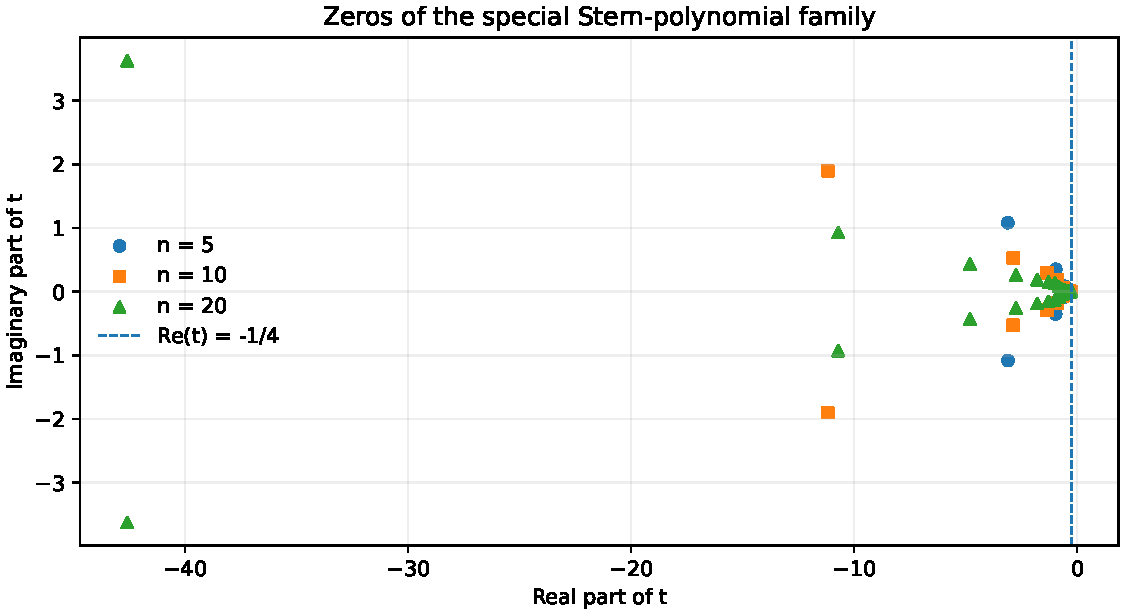
\includegraphics[width=0.92\textwidth]{figures/root_geometry.pdf}
 \caption{Numerical illustrations for $n=5,10,20$, obtained from the
 $n\times n$ tridiagonal matrices and their conjugates.  Points close to
 the real axis may appear to lie on it at this scale; \cref{thm:positive}
 excludes that possibility.  The dashed line is $\Repart t=-1/4$.
 Neither the plot nor floating-point eigenvalues are used in the proofs.}
 \label{fig:roots}
\end{figure}

\section{Generating functions and arithmetic consequences}\label{sec:arithmetic}

\subsection{Coefficient formulas and a rational generating function}

\begin{proposition}\label{prop:basic}
For $n\geq1$,
\begin{equation}\label{eq:Abinomial}
 A_n(t)=\sum_{j=0}^{n-1}\binom{2n-1-j}{j}t^j.
\end{equation}
Consequently,
\begin{equation}\label{eq:Wdegree}
 \deg W_n=2n,\qquad \lc(W_n)=n^2+n+1,\qquad W_n(0)=1.
\end{equation}
The degree and leading-coefficient formulas also hold at $n=0$.
\end{proposition}
\begin{proof}
Introduce Fibonacci polynomials $F_0=0$, $F_1=1$ and
$F_{m+2}=F_{m+1}+tF_m$.
Pascal's identity proves by induction that
\begin{equation}\label{eq:Fexplicit}
 F_m(t)=\sum_{j=0}^{\lfloor(m-1)/2\rfloor}
             \binom{m-1-j}{j}t^j\quad(m\geq1).
\end{equation}
Moreover,
\[
 F_{m+4}=(1+t)F_{m+2}+tF_{m+1}
         =(1+2t)F_{m+2}-t^2F_m.
\]
The subsequence $F_{2n}$ therefore satisfies the same recurrence and initial
values as $A_n$, so $A_n=F_{2n}$ and \eqref{eq:Abinomial} follows.
Its leading coefficient is $\binom{n}{n-1}=n$.
The degree-$2n$ coefficient of \eqref{eq:norm} is
\[
 (n+1)^2-n(n+1)+n^2=n^2+n+1>0.
\]
The constant coefficient and the case $n=0$ are immediate.
\end{proof}

There is also a useful nonrecursive square-minus-monomial formula.

\begin{proposition}\label{prop:squareminus}
For every $n\geq0$,
\begin{equation}\label{eq:squareminus}
 W_n(t)=(1+t)F_{2n+1}(t)^2-t^{2n+1}.
\end{equation}
In particular, $W_n(-1)=1$.
\end{proposition}
\begin{proof}
Cassini's identity for these Fibonacci polynomials is
\[
 F_{m+1}F_{m-1}-F_m^2=(-1)^m t^{m-1}\quad(m\geq1).
\]
For completeness, its left side at $m=1$ is $-1$, and replacing $m$ by
$m+1$ multiplies it by $-t$, as follows by substituting
$F_{m+2}=F_{m+1}+tF_m$ and $F_{m+1}-F_m=tF_{m-1}$.
Take $m=2n+1$ and set $X=F_{m+1}=A_{n+1}$,
$Y=tF_{m-1}=tA_n$.  Then $X-Y=F_m$ and
$XY=tF_m^2-t^m$ by Cassini.  Equation \eqref{eq:norm} becomes
\[
 W_n=X^2-XY+Y^2=(X-Y)^2+XY=(1+t)F_m^2-t^m.
\]
Substituting $t=-1$ finishes the proof.
\end{proof}

Let $u$ be a second formal variable.  The generating function across the
selected Stern indices is particularly small:
\begin{theorem}\label{thm:gf}
In $\Z[t][[u]]$,
\begin{equation}\label{eq:GF}
 \boxed{\quad
 \sum_{n\geq0}W_n(t)u^n
 =\frac{1-tu+t^4u^2}
 {1-(3t^2+4t+1)u+t^2(3t^2+4t+1)u^2-t^6u^3}.
 \quad}
\end{equation}
The denominator factors as
\[
 (1-t^2u)\bigl(1-(2t^2+4t+1)u+t^4u^2\bigr).
\]
\end{theorem}
\begin{proof}
Put $a=1+2t$ and consider
\[
 V_n=\begin{pmatrix}A_{n+1}^2\\A_{n+1}A_n\\A_n^2\end{pmatrix},
 \qquad
 V_{n+1}=S V_n,\qquad
 S=\begin{pmatrix}
 a^2&-2at^2&t^4\\a&-t^2&0\\1&0&0
 \end{pmatrix}.
\]
The characteristic polynomial of $S$ is
\[
 (\lambda-t^2)\bigl(\lambda^2-(2t^2+4t+1)\lambda+t^4\bigr).
\]
Cayley--Hamilton, followed by the linear functional $(1,-t,t^2)$,
therefore gives, with $p=3t^2+4t+1$,
\begin{equation}\label{eq:Wrecurrence}
 W_n=pW_{n-1}-t^2pW_{n-2}+t^6W_{n-3}\quad(n\geq3).
\end{equation}
This recurrence also appears in \cite{Ulas}; the argument here checks it
without using the initial polynomials printed there.
Direct computation from \eqref{eq:norm} gives
\begin{align*}
 W_0&=1,\\
 W_1&=1+3t+3t^2,\\
 W_2&=1+7t+17t^2+17t^3+7t^4.
\end{align*}
Multiplication of the formal series by the denominator in \eqref{eq:GF}
leaves the coefficients $1$, $W_1-pW_0=-t$, and
$W_2-pW_1+t^2pW_0=t^4$ in degrees zero, one, and two; all higher
coefficients vanish by \eqref{eq:Wrecurrence}.  This proves the formula
as a formal identity, including all exceptional values of $t$.
\end{proof}

\subsection{Exact reduction modulo three}

Define Lucas polynomials by
\[
 L_0=2,\qquad L_1=1,\qquad L_{m+2}=L_{m+1}+tL_m.
\]
For $m\geq1$, the recurrence and initial values show that
\begin{equation}\label{eq:LucasF}
 L_m=F_{m+1}+tF_{m-1}.
\end{equation}
For odd $m=2k+1$, this polynomial has degree $k$ and leading coefficient
$2k+1=m$: the two top coefficients on the right side are $k+1$ and $k$.
This includes $m=1$.

Write $\overline P$ for the reduction of $P\in\Z[t]$ in $\F_3[t]$.

\begin{theorem}\label{thm:mod3}
Let $n\geq0$, and write $2n+1=3^r v$ with $3\nmid v$.
Then
\begin{equation}\label{eq:mod3exact}
 \overline{W_n}=\overline{L_v}^{\,2\cdot3^r},\qquad
 \deg\overline{W_n}=2n+1-3^r.
\end{equation}
The reduced polynomial is monic.  In particular,
\begin{equation}\label{eq:mod3iff}
 \boxed{\quad W_n\equiv1\pmod3
 \quad\Longleftrightarrow\quad
 2n+1\text{ is a power of }3.\quad}
\end{equation}
Here $3^0=1$ is allowed.
\end{theorem}
\begin{proof}
In characteristic three, $-1=2$.  Thus \eqref{eq:norm} and
\eqref{eq:LucasF} give
\begin{equation}\label{eq:mod3square}
 \overline{W_n}
 =\bigl(\overline{A_{n+1}}+t\overline{A_n}\bigr)^2
 =\overline{L_{2n+1}}^{\,2}.
\end{equation}
The polynomial identity
\begin{equation}\label{eq:LucasFrobenius}
 L_{3m}=L_m^3-3(-t)^mL_m
\end{equation}
follows by writing $L_m=\alpha^m+\beta^m$ in the splitting field of
$X^2-X-t$, where $\alpha\beta=-t$, and expanding the cube.  Both sides
are integer polynomials, so it is an identity in $\Z[t]$.
Modulo three it gives $\overline{L_{3m}}=\overline{L_m}^{\,3}$.
Iteration and \eqref{eq:mod3square} prove the first formula in
\eqref{eq:mod3exact}.

Since $v$ is odd and not divisible by three, the top coefficient $v$
of $L_v$ survives reduction.  Therefore
\[
 \deg\overline{W_n}
 =2\cdot3^r\frac{v-1}{2}=3^r(v-1)=2n+1-3^r.
\]
Its leading coefficient is $v^{2\cdot3^r}=1$ in $\F_3$.
The reduced polynomial is constant exactly when $v=1$, and in that case
$L_v=L_1=1$.  This proves \eqref{eq:mod3iff}.
\end{proof}

The forward construction $n=(3^r-1)/2\Rightarrow W_n\equiv1\pmod3$
is a result of Ulas \cite[Theorem 3.1]{Ulas}.
The argument above independently proves it and also supplies the converse
and the exact degree drop within this family.

\subsection{An infinite irreducible subsequence}

\begin{corollary}\label{cor:irreducible}
For every $r\geq1$, with $n=(3^r-1)/2$, the polynomial $W_n$ is
irreducible in $\Q[t]$ and has degree $3^r-1$.
\end{corollary}
\begin{proof}
By \cref{thm:mod3}, every nonconstant coefficient of $W_n$ is divisible
by three, whereas its constant coefficient is one.
The leading coefficient from \cref{prop:basic} is
\[
 n^2+n+1=\frac{3^{2r}+3}{4}
         =3\,\frac{3^{2r-1}+1}{4}.
\]
It is divisible by three but not nine, since $3^{2r-1}+1\equiv1\pmod3$
and $4$ is a unit modulo three.
The reciprocal polynomial
\[
 R_n(t)=t^{2n}W_n(1/t)
\]
is therefore monic, all its nonleading coefficients are divisible by three,
and its constant coefficient is not divisible by nine.
Eisenstein's criterion at three makes $R_n$ irreducible over $\Q$.
Because $W_n(0)=1$, taking reciprocals carries any nontrivial factorization
of $W_n$ to a nontrivial factorization of $R_n$; hence $W_n$ is irreducible.

For completeness, the relevant Eisenstein argument is elementary.
By Gauss's lemma, a rational factorization of a monic integer polynomial
can be taken monic with integer coefficients.  Reduction of $R_n$ modulo
three is $t^{2n}$, so the reductions of two positive-degree monic factors
would both be powers of $t$.  Both constant coefficients would be divisible
by three, forcing the constant coefficient of $R_n$ to be divisible by nine,
a contradiction.
\end{proof}

This does not assert irreducibility for every $n$.  The indices
$n=1,4,13,40,121,364,\ldots$ form the proven subsequence.

\section{Asymptotic nonreal zeros}\label{sec:asymptotic}

The matrix enclosure permits $|t|$ of order $n^2$.  We next show that this
scale actually occurs, with imaginary parts of order $n$.
The unboundedness of imaginary parts across all Stern polynomials is
already known \cite[Theorem 10]{Altizio}; the result here is an explicit
asymptotic for the particular family selected in \cref{sec:target}.

\begin{theorem}\label{thm:asymptotic}
Fix an integer $j\geq1$.  For all sufficiently large $n$, there is a zero
$t_{n,j}$ of $W_n$ in the lower half-plane such that, with
$\zeta=(1+i\sqrt3)/2$,
\begin{equation}\label{eq:rootasymp}
 \boxed{\quad
 t_{n,j}=-\frac{(n+\zeta)^2}{j^2\pi^2}-\frac1{12}
         -\frac{i\sqrt3}{3(n+\zeta)}+O_j(n^{-2}).
 \quad}
\end{equation}
Its conjugate is also a zero.  In particular,
\begin{align}
 \Repart t_{n,j}&=-\frac{n^2+n-\frac12}{j^2\pi^2}
                      -\frac1{12}+O_j(n^{-2}),\label{eq:rootreal}\\
 \Impart t_{n,j}&=-\frac{\sqrt3(n+\frac12)}{j^2\pi^2}
                      +O_j(n^{-1}),\label{eq:rootimag}\\
 \frac{\Repart t_{n,j}}{(\Impart t_{n,j})^2}
                  &\longrightarrow-\frac{j^2\pi^2}{3}.\label{eq:parabolic}
\end{align}
The notation $O_j$ allows constants depending on the fixed integer $j$;
no estimate uniform in $1\leq j\leq n$ is asserted.
\end{theorem}
\begin{proof}
From \eqref{eq:Chebyshev}, or directly from the sine addition formula,
\[
 C_n(2\cos\theta)=\frac{\sin((n+1)\theta)}{\sin\theta}
\]
whenever $\sin\theta\neq0$.
The factor $C_n-\zeta C_{n-1}$ therefore vanishes if
\begin{equation}\label{eq:quantization}
 \sin((n+1)\theta)-\zeta\sin(n\theta)=0.
\end{equation}
Near zero, define the analytic function
\begin{equation}\label{eq:delta}
 \delta(\theta)=\arctan\left(\frac{\sin\theta}{\cos\theta-\zeta}\right),
 \qquad \delta(0)=0,
\end{equation}
using the local branch of $\arctan$ at zero.
The denominator is nonzero there because $1-\zeta\neq0$.
By the sine addition formula, \eqref{eq:quantization} is equivalent,
in a sufficiently small neighborhood, to
\[
 \sin(n\theta+\delta(\theta))=0.
\]
Indeed, multiplying its left side by
$(\cos\theta-\zeta)/\cos\delta(\theta)$ gives exactly the left side of
\eqref{eq:quantization}; the multiplier is nonzero near zero.

To construct the required root rigorously, put $\varepsilon=1/n$ and
$\theta=\varepsilon u$.  The equation
\[
 u+\delta(\varepsilon u)=j\pi
\]
has a unique analytic solution $u=u(\varepsilon)$ near
$(u,\varepsilon)=(j\pi,0)$, by the analytic implicit function theorem:
the derivative with respect to $u$ there is one.
For positive integers $n$ sufficiently large,
$\theta_n=u(1/n)/n$ is small and nonzero, so $\sin\theta_n\neq0$.
Consequently \eqref{eq:quantization} gives an actual zero of the polynomial
factor, not a spurious zero caused by the sine denominator.

We now compute the expansion.  The identities
$(1-\zeta)^{-1}=\zeta$, $\zeta^2=\zeta-1$, and $\zeta^3=-1$ give
\begin{align*}
 \delta(\theta)
  &=\zeta\theta+
       \left(\frac{\zeta^2}{2}-\frac\zeta6-\frac{\zeta^3}{3}\right)
           \theta^3+O(\theta^5)\\
  &=\zeta\theta+\frac{i\sqrt3}{6}\theta^3+O(\theta^5).
\end{align*}
Write $N=n+\zeta$, $q=j\pi$, and $c=i\sqrt3/6$.
The equation $n\theta_n+\delta(\theta_n)=q$, together with
$\theta_n=O_j(n^{-1})$, now yields
\[
 \theta_n=\frac qN-\frac{c q^3}{N^4}+O_j(n^{-6}),\qquad
 \frac1{\theta_n^2}=\frac{N^2}{q^2}+\frac{2c}{N}+O_j(n^{-3}).
\]
For example, the first estimate follows by first obtaining
$\theta_n=q/N+O_j(n^{-4})$ and substituting this back into the cubic term;
the remainder $O(\theta_n^5)$ contributes $O_j(n^{-6})$ after division
by $N$.

The corresponding zero in the original variable is
\[
 t_{n,j}=\frac1{2\cos\theta_n-2}
        =-\frac1{4\sin^2(\theta_n/2)}
        =-\frac1{\theta_n^2}-\frac1{12}+O(\theta_n^2).
\]
Substitution proves \eqref{eq:rootasymp}.  Its imaginary part is negative
for sufficiently large $n$, consistently with \cref{thm:enclosure}.
Since $W_n$ has real coefficients, the conjugate is a zero as well.
Taking real and imaginary parts gives \eqref{eq:rootreal} and
\eqref{eq:rootimag}; the real part of $-i\sqrt3/(3N)$ is $O(n^{-2})$.
Finally, division of the leading terms gives \eqref{eq:parabolic}.
\end{proof}

The asymptotic is more informative than the mere existence of nonreal
zeros.  Along these branches the distance from the real axis grows
unboundedly, even though the angle to the negative real axis tends to zero.
It also shows why a search restricted to a fixed rectangular window in the
complex plane would miss some of the most distinctive roots.

\section{Computational audit and reproducibility}\label{sec:computation}

The universal results in this note rest on the proofs, not on a finite
search.  The programs are included to make indexing mistakes, coefficient
errors, and numerical overinterpretation easier to detect.
The primary exact evaluator constructs $(B_m,B_{m+1})$ directly from the
binary digits of $m$:
\[
 (P,Q)\stackrel{0}{\longmapsto}(tP,P+Q),\qquad
 (P,Q)\stackrel{1}{\longmapsto}(P+Q,tQ),\qquad (P,Q)=(0,1)\text{ initially}.
\]
This route is independent of the second-order recurrence for $A_n$ and of
the quadratic formula for $W_n$.  The latter formulas are tested against it,
not used to define the purported ground truth.

\subsection{Exact checks actually executed}

The delivered \texttt{code/verify\_exact.py} uses only the Python standard
library, integer coefficient arrays, and rational Sturm remainders.
The recorded run used Python 3.13.5 and passed \textbf{6,722 checks}.
The scope is summarized in \cref{tab:checks}.  Counts refer to individual
assertions, not to distinct conjectures or independently formalized proofs.

\begin{table}[htb]
\centering\small
\begin{tabular}{@{}>{\raggedright\arraybackslash}p{0.51\textwidth}>{\raggedright\arraybackslash}p{0.39\textwidth}@{}}
\toprule
Check & Executed range or extent\\
\midrule
Binary evaluator against the direct Stern recurrence & Indices $0\leq m\leq1024$\\
Hyperbinary generating product against $B_{m+1}$ & Coefficients $0\leq m\leq64$ in $x$\\
Concatenation, including both endpoints & $0\leq k\leq6$, $0\leq m\leq24$, $0\leq r\leq2^k$\\
Three constructions of $A_n$; adjacent conversion & $0\leq n\leq160$\\
Quadratic, sum-of-squares, and square-minus-monomial identities & $0\leq n\leq160$\\
Degree, leading coefficient, reduction modulo three & $0\leq n\leq160$\\
Third-order recurrence and generating-function numerator & $3\leq n\leq160$; initial two coefficients\\
Reciprocal Eisenstein conditions & $r=1,\ldots,6$; maximum $n=364$, degree $728$\\
Exact rational Sturm counts, with control examples & $n=1,\ldots,12$; zero real roots in every case\\
\bottomrule
\end{tabular}
\caption{The exact finite audit.  Full assertion counts and sample
coefficients are stored in \texttt{results/exact\_verification.json}.}
\label{tab:checks}
\end{table}

The largest Eisenstein case was also checked against a direct Stern-index
evaluation, rather than only against the abstract congruence criterion.
Sturm counts are exact over $\Q$; they do not rely on small imaginary
parts returned by a floating-point root finder.

\subsection{Numerical illustrations}

The optional script \texttt{code/numerical\_checks.py} computes matrix
eigenvalues for seven values of $n$ up to $100$, and tests the displayed
spectral inequalities numerically.  It also solves the sine equation at
80 decimal digits for $j=1,2$ and $n=10,20,50,100,200,500$.
Each result is cross-checked by evaluating the polynomial recurrence
$C_n-\zeta C_{n-1}$, with the normalized residual required to be less
than $10^{-65}$.  This is a numerical diagnostic, not interval-certified
root isolation.

Let
\[
 T_{n,1}^{(0)}=-\frac{(n+\zeta)^2}{\pi^2}-\frac1{12}.
\]
For the lower root with $j=1$, the observed values in \cref{tab:asymptotic}
illustrate the proven first correction:
$n|t_{n,1}-T_{n,1}^{(0)}|\to\sqrt3/3$.
This limit itself follows from \eqref{eq:rootasymp}; it is not inferred
from the table.

\begin{table}[htb]
\centering\small
\begin{tabular}{@{}rrrr@{}}
\toprule
$n$ & $\Repart t_{n,1}$ & $\Impart t_{n,1}$ &
 $n|t_{n,1}-T_{n,1}^{(0)}|$\\
\midrule
10 & $-11.18381641$ & $-1.89989755$ & $0.57511034$\\
20 & $-42.58891626$ & $-3.62608332$ & $0.56999317$\\
50 & $-258.40190478$ & $-8.87387171$ & $0.57275425$\\
100 & $-1023.37668120$ & $-17.64283788$ & $0.57476199$\\
200 & $-4073.14426863$ & $-35.18931419$ & $0.57598204$\\
500 & $-25380.98917731$ & $-87.83561926$ & $0.57678499$\\
\bottomrule
\end{tabular}
\caption{Rounded numerical data.  The limiting value in the last column
is $\sqrt3/3\approx0.57735027$.  Higher precision and the refined-error
columns are in \texttt{results/root\_asymptotics.csv}.}
\label{tab:asymptotic}
\end{table}

\subsection{How to reproduce the archive}

From the extracted archive directory, run
\begin{verbatim}
python3 code/verify_exact.py
pdflatex -interaction=nonstopmode -halt-on-error stern_conjecture_note.tex
pdflatex -interaction=nonstopmode -halt-on-error stern_conjecture_note.tex
\end{verbatim}
The optional numerical script requires \texttt{mpmath}, \texttt{numpy}, and
\texttt{matplotlib}. Installation details are in
\texttt{requirements-optional.txt}.
The figure PDF is included, so rebuilding the note does not require these
optional packages.  No program needs a network connection.

\section{What has and has not been established}\label{sec:limits}

The selected assertion is proved for every allowed index and every real
argument, with no numerical hypothesis.  The stronger complex-zero
localization, the generating function, the exact reduction-modulo-three
criterion, the infinite irreducible subsequence, and the fixed-$j$ root
asymptotic likewise have unconditional proofs within this note.

There are separate limits to the claim.  The targeted literature search is
not a proof of priority, and it did not verify the final journal version
of the 2019 conjecture.  The current write-up has not received external
mathematical review.  The code provides a finite audit, not a formal proof
of the universal statements.  Finally, none of the arguments here resolves
the zero geometry or irreducibility of \emph{all} Stern polynomials.

The central mathematical lesson is a specific structural one.  The sparse
binary indices $h_n$ lead to a quadratic form in two nearby auxiliary
polynomials.  Once that form is written correctly, its discriminant is
$-3t^2$, and the real-zero question reduces to a one-line backward-recursion
argument.  The same form then exposes both an Eisenstein norm and a
tridiagonal boundary perturbation, explaining why arithmetic and spectral
consequences emerge from the same certificate.

\appendix
\section{Source audit for the arXiv version}\label{sec:audit}

The following corrections concern only \texttt{arXiv:1909.10844v1}, whose
PDF pages 13, 14, and 16 were visually checked.  They are not assertions
about the final journal typesetting.

On page 13, the adjacent-polynomial identity is consistent with
\eqref{eq:adjquadratic}.  After the displayed substitution for
$B_{a_n+1}$, however, the quadratic in $(X,Y)=(A_n,A_{n+1})$ must be
\[
 F(X,Y)=t^2X^2-tXY+Y^2,
\]
not the expression printed there.
On page 14, the initial values compatible with the Stern definition are
\[
 W_1=3t^2+3t+1,\qquad
 W_2=7t^4+17t^3+17t^2+7t+1.
\]
The coefficients of $t$ in $W_1$ and $t^2$ in $W_2$ differ from those
printed in the arXiv recurrence display.  The third-order recurrence itself
is consistent with the independent derivation in \cref{thm:gf}.

These observations are checks on the formulas actually used, not an attempt
to audit every statement of the source.  The proof in this note starts from
\eqref{eq:stern} and does not depend on adopting any corrected formula
on authority.

\section{Small exact examples}\label{sec:examples}

The first auxiliary polynomials are
\begin{align*}
 A_0&=0,& A_1&=1,& A_2&=1+2t,\\
 A_3&=1+4t+3t^2,&
 A_4&=1+6t+10t^2+4t^3.
\end{align*}
The first nonconstant members of the target family are
\begin{align*}
 W_1={}&1+3t+3t^2,\\
 W_2={}&1+7t+17t^2+17t^3+7t^4,\\
 W_3={}&1+11t+47t^2+99t^3+108t^4+58t^5+13t^6,\\
 W_4={}&1+15t+93t^2+309t^3+597t^4\\
       &\quad+681t^5+444t^6+150t^7+21t^8.
\end{align*}
For example,
\[
 W_1=(1+2t)^2-t(1+2t)+t^2=1+3t+3t^2,
\]
and its zeros are $-1/2\pm i\sqrt3/6$.
The cases $n=1$ and $n=4$ have $2n+1=3,9$; every nonconstant coefficient
is divisible by three, and their leading coefficients $3$ and $21$ are
not divisible by nine, as required by \cref{cor:irreducible}.

\begin{thebibliography}{9}
\bibitem{KMP}
S.~Klav\v{z}ar, U.~Milutinovi\'{c}, and C.~Petr,
\emph{Stern polynomials},
Advances in Applied Mathematics \textbf{39} (2007), 86--95.
Author-hosted preprint:
\url{https://users.fmf.uni-lj.si/klavzar/preprints/SternPolyFinal.pdf}.

\bibitem{Ulas}
M.~Ulas,
\emph{Strong arithmetic property of certain Stern polynomials},
Publicationes Mathematicae Debrecen \textbf{96} (2020), 401--422.
\href{https://doi.org/10.5486/PMD.2020.8683}{doi:10.5486/PMD.2020.8683}.
The text and conjecture numbering checked in this note are those of
\href{https://arxiv.org/abs/1909.10844v1}{arXiv:1909.10844v1},
24 September 2019.  The final journal PDF was not inspected.

\bibitem{Altizio}
D.~Altizio,
\emph{Zeros of Stern polynomials in the complex plane},
\href{https://arxiv.org/abs/2511.03847v1}{arXiv:2511.03847v1},
5 November 2025.
\end{thebibliography}

\end{document}
